\documentclass{beamer}
\usepackage[utf8]{inputenc}

\usetheme{Madrid}
\usecolortheme{default}
\usepackage{amsmath,amssymb,amsfonts,amsthm}
\usepackage{txfonts}
\usepackage{tkz-euclide}
\usepackage{listings}
\usepackage{adjustbox}
\usepackage{array}
\usepackage{tabularx}
\usepackage{gvv}
\usepackage{gvv}
\usepackage{lmodern}
\usepackage{circuitikz}
\usepackage{tikz}
\usepackage{graphicx}

\setbeamertemplate{page number in head/foot}[totalframenumber]

\usepackage{tcolorbox}
\tcbuselibrary{minted,breakable,xparse,skins}



\definecolor{bg}{gray}{0.95}
\DeclareTCBListing{mintedbox}{O{}m!O{}}{%
  breakable=true,
  listing engine=minted,
  listing only,
  minted language=#2,
  minted style=default,
  minted options={%
    linenos,
    gobble=0,
    breaklines=true,
    breakafter=,,
    fontsize=\small,
    numbersep=8pt,
    #1},
  boxsep=0pt,
  left skip=0pt,
  right skip=0pt,
  left=25pt,
  right=0pt,
  top=3pt,
  bottom=3pt,
  arc=5pt,
  leftrule=0pt,
  rightrule=0pt,
  bottomrule=2pt,
  toprule=2pt,
  colback=bg,
  colframe=orange!70,
  enhanced,
  overlay={%
    \begin{tcbclipinterior}
    \fill[orange!20!white] (frame.south west) rectangle ([xshift=20pt]frame.north west);
    \end{tcbclipinterior}},
  #3,
}
\lstset{
    language=C,
    basicstyle=\ttfamily\small,
    keywordstyle=\color{blue},
    stringstyle=\color{orange},
    commentstyle=\color{green!60!black},
    numbers=left,
    numberstyle=\tiny\color{gray},
    breaklines=true,
    showstringspaces=false,
}
%------------------------------------------------------------
%This block of code defines the information to appear in the
%Title page
\title %optional
{2.10.77}
\date{}
%\subtitle{A short story}

\author % (optional)
{Sai Krishna Bakki - EE25BTECH11049}



\begin{document}


\frame{\titlepage}
\begin{frame}{Question}
The points $(-a, -b)$, $(0, 0)$, $(a, b)$ and $(a^2, ab)$ are
\begin{enumerate}
\item Collinear
\item Vertices of a parallelogram
\item Vertices of a rectangle
\item None of these
\end{enumerate}
\end{frame}

\begin{frame}{Checking For The Points To Be Vertices Of A Parallelogram}
    \begin{align}
\vec{A}=\myvec{-a\\-b},\vec{B}=\myvec{0\\0},\vec{C}=\myvec{a\\b},\vec{D}=\myvec{a^2\\ab}
\end{align}
Condition for the points to be vertices of a parallelogram is \\
\begin{align}
    \vec{B}-\vec{A}=\vec{C}-\vec{D}\\
    \vec{B}-\vec{A}=\myvec{a\\b},\vec{C}-\vec{D}=\myvec{a-a^2\\b-ab}
\end{align}
But
\begin{align}
\vec{B}-\vec{A} \neq \vec{C}-\vec{D}
\end{align} 
If
$\vec{B}-\vec{A} \neq \vec{C}-\vec{D}$ then the points cannot be vertices of a rectangle too because every rectangle is a specific type of parallelogram.
\end{frame}
\begin{frame}{Checking For The Points To Be Collinear}
    Condition for the points to be collinear is
\begin{align}
    \text{rank}\myvec{\vec{B} - \vec{A} & &\vec{C} - \vec{D}} = 1\\
\end{align}
\begin{align}
    \text{rank}\myvec{a & a-a^2\\b & b-ab}
\end{align}
By transformation $R_2 \rightarrow \frac{-b}{a}R_2 + 2R_1$
\begin{align}
    \text{rank}\myvec{a & a-a^2 \\ 0 & 0} =1
\end{align}
The number of non zero rows in the row reduced matrix (also known as {\em echelon form}) is defined as the rank.\\
For the above matrix, Rank is one.\\
Therefore, we can conclude that four points are collinear.

\end{frame}
\begin{frame}[fragile]
\frametitle{C Code }
\begin{lstlisting}
#include <stdio.h>
#ifdef __cplusplus
extern "C" {
#endif

    double check_collinearity(double x1, double y1, double x2, double y2, double x3, double y3) {
        // Calculate the determinant
        double determinant = x1 * (y2 - y3) + x2 * (y3 - y1) + x3 * (y1 - y2);
        return determinant;
    }

#ifdef __cplusplus
}
#endif
\end{lstlisting}
\end{frame}
\begin{frame}[fragile]
\frametitle{Python Code through shared output}
\begin{lstlisting}
# Code by GVV Sharma
# September 12, 2023
# released under GNU GPL
# This script checks if the points (-a,-b), (0,0), (a,b), and (a^2, ab) are collinear.

import numpy as np
import numpy.linalg as LA
import matplotlib.pyplot as plt
import subprocess
import shlex
import ctypes
import os

# local imports (assuming funcs.py is in the same directory)
from libs.funcs import *

# --- COMPILE AND LOAD C FUNCTION ---
# This block compiles line.c into a shared library and loads it.
\end{lstlisting}
\end{frame}
\begin{frame}[fragile]
\frametitle{Python Code through shared output}
\begin{lstlisting}
c_file = "line.c"
lib_file = "line.so" if os.name != 'nt' else "line.dll"

# Compile C code into a shared library
# The -fPIC flag is needed for creating a shared library
compile_command = f"gcc -shared -o {lib_file} -fPIC {c_file}"
try:
    subprocess.run(shlex.split(compile_command), check=True)
    print(f"Successfully compiled {c_file} to {lib_file}\n")
except (subprocess.CalledProcessError, FileNotFoundError):
    print("Error: C compilation failed. Make sure gcc is installed and in your PATH.")
    exit()

# Load the shared library
try:
    c_lib = ctypes.CDLL(os.path.abspath(lib_file))
    \end{lstlisting}
\end{frame}
\begin{frame}[fragile]
\frametitle{Python Code through shared output}
\begin{lstlisting}
except OSError as e:
    print(f"Error loading shared library: {e}")
    exit()

# Define the C function's signature (argument types and return type)
check_collinearity_c = c_lib.check_collinearity
check_collinearity_c.argtypes = [ctypes.c_double] * 6  # six double arguments
check_collinearity_c.restype = ctypes.c_double         # returns a double

# --- PROBLEM SETUP ---

# For a tangible example, let's choose non-zero values for a and b
a = 2.0
b = 3.0
\end{lstlisting}
\end{frame}
\begin{frame}[fragile]
\frametitle{Python Code through shared output}
\begin{lstlisting}
# Define the four points using numpy arrays
P1 = np.array([-a, -b]).reshape(-1, 1)
P2 = np.array([0.0, 0.0]).reshape(-1, 1)
P3 = np.array([a, b]).reshape(-1, 1)
P4 = np.array([a**2, a*b]).reshape(-1, 1)

# --- METHOD 1: MATRIX RANK COLLINEARITY CHECK (Original Method) ---
print("--- Method 1: NumPy Matrix Rank ---")
# Form a matrix with the vectors as columns.
vec_matrix = np.hstack([P1, P3, P4])
rank = LA.matrix_rank(vec_matrix)

print(f"Checking points with a={a}, b={b}")
print(f"Matrix of vectors (from origin to other points):\n{vec_matrix}")
print(f"Rank of the matrix: {rank}")
\end{lstlisting}
\end{frame}
\begin{frame}[fragile]
\frametitle{Python Code through shared output}
\begin{lstlisting}
if rank == 1:
    print("Conclusion: A rank of 1 means the points are COLLINEAR. ✅")
else:
    print("Conclusion: The points are NOT collinear. ❌")

print("-" * 40)

# --- METHOD 2: C FUNCTION COLLINEARITY CHECK (New Method) ---
print("--- Method 2: Calling C function via ctypes ---")
# To check if 4 points are collinear, we can check 2 sets of 3 points.
# For example, are P1, P2, P3 collinear? And are P1, P2, P4 collinear?

# Check collinearity for points P1, P2, and P3
det1 = check_collinearity_c(
\end{lstlisting}
\end{frame}
\begin{frame}[fragile]
\frametitle{Python Code through shared output}
\begin{lstlisting}
    P1[0,0], P1[1,0],  # P1(x, y)
    P2[0,0], P2[1,0],  # P2(x, y)
    P3[0,0], P3[1,0]   # P3(x, y)
)

# Check collinearity for points P1, P2, and P4
det2 = check_collinearity_c(
    P1[0,0], P1[1,0],  # P1(x, y)
    P2[0,0], P2[1,0],  # P2(x, y)
    P4[0,0], P4[1,0]   # P4(x, y)
)

print(f"Determinant for P1, P2, P3: {det1}")
print(f"Determinant for P1, P2, P4: {det2}")

# For floating point numbers, check if the determinant is very close to zero
if abs(det1) < 1e-9 and abs(det2) < 1e-9:
\end{lstlisting}
\end{frame}
\begin{frame}[fragile]
\frametitle{Python Code through shared output}
\begin{lstlisting}
    print("\nConclusion: Both determinants are zero, so the points are COLLINEAR.")
else:
    print("\nConclusion: At least one determinant is non-zero, so the points are NOT collinear.")

# --- PLOTTING SECTION (No changes needed here) ---
print("\nGenerating plot...")
x_line = line_gen(P1, P4)
plt.plot(x_line[0,:], x_line[1,:], label='Line of Collinearity')
all_coords = np.hstack([P1, P2, P3, P4])
plt.scatter(all_coords[0,:], all_coords[1,:])
vert_labels = ['P1(-a, -b)', 'P2(0, 0)', 'P3(a, b)', 'P4(a², ab)']
for i, txt in enumerate(vert_labels):
    plt.annotate(f'{txt}\n({all_coords[0,i]:.1f}, {all_coords[1,i]:.1f})',
                 (all_coords[0,i], all_coords[1,i]),
                 textcoords="offset points", xytext=(0,10), ha='center')
\end{lstlisting}
\end{frame}
\begin{frame}[fragile]
\frametitle{Python Code through shared output}
\begin{lstlisting}
ax = plt.gca()
ax.spines['top'].set_color('none')
ax.spines['left'].set_position('zero')
ax.spines['right'].set_color('none')
ax.spines['bottom'].set_position('zero')
plt.legend(loc='best')
plt.grid()
plt.axis('equal')
plt.show()

# Clean up the compiled library file
if os.path.exists(lib_file):
    os.remove(lib_file)
\end{lstlisting}
\end{frame}
\begin{frame}[fragile]
\frametitle{Python Code}
\begin{lstlisting}
# Code by GVV Sharma
# September 12, 2023
# Revised September 28, 2025
# released under GNU GPL
# This script checks if the points (-a,-b), (0,0), (a,b), and (a^2, ab) are collinear.

import sys                                        
import numpy as np
import numpy.linalg as LA
import matplotlib.pyplot as plt

# local imports
from libs.funcs import *

# if using termux
import subprocess
import shlex
# end if
\end{lstlisting}
\end{frame}
\begin{frame}[fragile]
\frametitle{Python Code}
\begin{lstlisting}
# For a tangible example, let's choose non-zero values for a and b
a = 2
b = 3

# Define the four points based on the problem statement
P1 = np.array([-a, -b]).reshape(-1, 1)
P2 = np.array([0, 0]).reshape(-1, 1)
P3 = np.array([a, b]).reshape(-1, 1)
P4 = np.array([a**2, a*b]).reshape(-1, 1)

# To check if all points are collinear, we can check the rank of a matrix
# formed by the vectors from the origin (P2) to the other points.
# The vectors are P1-P2 (i.e., P1), P3-P2 (i.e., P3), and P4-P2 (i.e., P4).
# If all these vectors lie on the same line, the rank of the matrix will be 1.
\end{lstlisting}
\end{frame}
\begin{frame}[fragile]
\frametitle{Python Code}
\begin{lstlisting}
# Form a matrix with the vectors as columns
# Note: P2 is the origin, so it's not needed to form the vectors.
vec_matrix = np.block([P1, P3, P4])

# Calculate and print the rank
rank = LA.matrix_rank(vec_matrix)
print(f"The points are defined with a={a} and b={b}")
print(f"Matrix of vectors:\n{vec_matrix}")
print(f"Rank of the matrix: {rank}")

if rank == 1:
    print("Conclusion: A rank of 1 means the vectors are linearly dependent, so the points are COLLINEAR. ✅")
else:
    print("Conclusion: The points are NOT collinear. ❌")


# --- Plotting Section ---
\end{lstlisting}
\end{frame}
\begin{frame}[fragile]
\frametitle{Python Code}
\begin{lstlisting}
# Generate a line passing through the points to visualize.
# We can use the two outer points, P1 and P4, to draw the line.
x_line = line_gen(P1, P4)

# Plot the generated line
plt.plot(x_line[0,:], x_line[1,:], label='Line of Collinearity')

# Combine all points into one array for plotting
all_coords = np.block([[P1, P2, P3, P4]])
plt.scatter(all_coords[0,:], all_coords[1,:])

# Label the coordinates
vert_labels = ['P1(-a, -b)', 'P2(0, 0)', 'P3(a, b)', 'P4(a², ab)']
for i, txt in enumerate(vert_labels):
    plt.annotate(f'{txt}\n({all_coords[0,i]:.0f}, {all_coords[1,i]:.0f})',
 (all_coords[0,i], all_coords[1,i]), # Point to label
 \end{lstlisting}
\end{frame}
\begin{frame}[fragile]
\frametitle{Python Code}
\begin{lstlisting}
 textcoords="offset points",   # How to position the text
 xytext=(0,10),           # Distance from text to points (x,y)
    ha='center')                  # Horizontal alignment

# use set_position
ax = plt.gca()
ax.spines['top'].set_color('none')
ax.spines['left'].set_position('zero')
ax.spines['right'].set_color('none')
ax.spines['bottom'].set_position('zero')
plt.legend(loc='best')
plt.grid()
plt.axis('equal')
plt.show()
\end{lstlisting}
\end{frame}
\begin{frame}{Plot By C code and Python Code}
    \begin{figure}
    \centering
    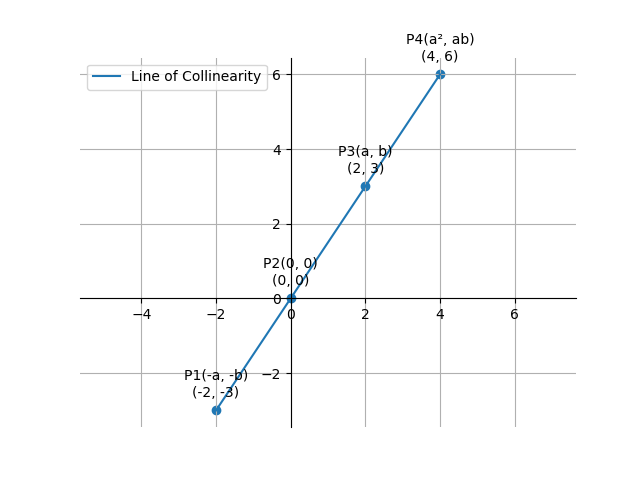
\includegraphics[width=0.7\columnwidth]{figs/Figure_1.png}
    \label{fig:placeholder}
    \caption{1}
\end{figure}
\end{frame}
\end{document}
